\documentclass[10pt,twocolumn]{article}

% ------------------------------------------------------------------ packages
\usepackage[letterpaper,top=0.9in,bottom=1in,left=0.75in,right=0.75in]{geometry}
\usepackage{newtxtext,newtxmath}
\usepackage{graphicx}
\usepackage{booktabs}
\usepackage{amsmath}
\usepackage{microtype}
\usepackage{xcolor}
\usepackage[font=small,labelfont=bf]{caption}
\usepackage{algorithm}
\usepackage{algpseudocode}
% Coherent, compact heading hierarchy: 12pt sections, 10pt bold subsections,
% run-in paragraph heads — no jumps in visual weight.
\usepackage{titlesec}
\titleformat{\section}{\large\bfseries}{\thesection}{0.6em}{}
\titleformat{\subsection}{\normalsize\bfseries}{\thesubsection}{0.6em}{}
\titleformat{\paragraph}[runin]{\normalsize\bfseries}{}{0em}{}[.]
\titlespacing*{\section}{0pt}{1.1em plus 0.3em}{0.5em}
\titlespacing*{\subsection}{0pt}{0.9em plus 0.2em}{0.4em}
\titlespacing*{\paragraph}{0pt}{0.7em plus 0.2em}{0.5em}
\usepackage[colorlinks=true,linkcolor=blue!60!black,citecolor=blue!60!black,urlcolor=blue!60!black]{hyperref}

\graphicspath{{figures/}}
\setlength{\columnsep}{0.28in}

% Allow several floats per page top so figure-dense sections do not spill pages.
\renewcommand{\topfraction}{0.92}
\renewcommand{\bottomfraction}{0.7}
\renewcommand{\textfraction}{0.06}
\renewcommand{\floatpagefraction}{0.8}
\setcounter{topnumber}{4}
\setcounter{totalnumber}{6}

\newcommand{\fromInit}{\texttt{arap\_from\_init}}
\newcommand{\iterMode}{\texttt{arap\_iterative}}
% Contrastive naming used in all figures, tables, and text:
%   "SC-GS (original)"  = the original paper's default one-shot editing mode (arap_from_init)
%   "Ours (N=k)"        = progressive drag scheduling with k sub-steps
%   "SC-GS iterative"   = the original slow incremental mode, used as robustness reference
\newcommand{\scgsOrig}{SC-GS (original)}
\newcommand{\ours}[1]{Ours ($N{=}#1$)}
\newcommand{\scgsIter}{SC-GS iterative}
\newcommand{\eg}{\emph{e.g.}}
\newcommand{\etal}{\emph{et al.}}
\newcommand{\ie}{\emph{i.e.}}

\title{\LARGE\bf Progressive Drag Scheduling: Characterizing and Repairing\\
Large-Rotation Editing Failures in Sparse-Controlled Gaussian Splatting}

\author{%
  \textit{$\langle$TODO: name, student ID$\rangle$}\\
  \textit{$\langle$TODO: department / major, laboratory$\rangle$}\\
  \textit{Own research topic: $\langle$TODO$\rangle$}\\
  Visual Media, The University of Tokyo\\[2pt]
  \small Code: \url{https://github.com/<TODO-user>/sc-gs-failure-analysis}}

\date{}

\begin{document}

\twocolumn[{%
\maketitle
\begin{abstract}
\noindent
Sparse-Controlled Gaussian Splatting (SC-GS) couples dense 3D Gaussians with a
sparse set of learned control points, enabling both high-fidelity dynamic
novel-view synthesis and interactive motion editing through as-rigid-as-possible
(ARAP) deformation of the control graph. We present a systematic empirical study
of when and why this editing pipeline fails. First, we show that the default
editing mode, which initializes every ARAP solve from a linear Laplacian-editing
solution, collapses for rotational drags beyond 45--60$^\circ$: the
rotation-blind initialization produces the classical chord-shortcut artifact,
and the fixed budget of three local-global iterations cannot recover from it,
yielding under-rotated, shortened limbs and torn Gaussian layouts. Second, we
identify two further failure axes: an initialization-independent artifact in the
rotation re-estimation stage that propagates node motion to Gaussians, and a
strong sensitivity of \emph{editability} --- but not reconstruction quality ---
to the number of control points, including a previously unreported global
``leakage'' failure at high control-point counts that local rigidity metrics
cannot detect. Motivated by this analysis, we propose \emph{progressive drag
scheduling}: a requested drag is subdivided into $N$ sub-steps along the target
trajectory, and each sub-step's ARAP solve is warm-started from the previous
solution. The method is a pure scheduling change --- it requires no modification
of the trained model or the solver --- yet it extends the failure-onset angle
from 45--60$^\circ$ to 90--110$^\circ$ ($N{=}8$) at under 0.8\,s per drag,
16$\times$ faster than the robust-but-slow incremental reference mode. Across
eight D-NeRF scenes spanning organic limbs, a mechanical hinge, an extreme
kinematic chain, and a free body, progressive scheduling closes 43--80\% of
the rigidity gap between the original and reference modes, with monotone
improvement in the schedule length on nearly every scene and angle. All
results are reproducible from committed scripts, metrics, and protocol seeds.

\vspace{0.6em}
\noindent\textbf{Keywords:} dynamic scene reconstruction; 3D Gaussian splatting;
sparse control points; as-rigid-as-possible deformation; interactive shape
editing; failure analysis; warm-start scheduling.
\end{abstract}
\vspace{1.0em}
}]

% =====================================================================
\section{Introduction}
\label{sec:intro}

Photorealistic reconstruction of dynamic scenes has advanced rapidly from neural
radiance fields~\cite{nerf,dnerf} to point-based representations built on 3D
Gaussian Splatting (3DGS)~\cite{3dgs}, which offer real-time rendering and
explicit geometry. Beyond replaying a captured sequence, a natural next demand
is \emph{editing}: a user should be able to grab a reconstructed character and
pose it --- bend an arm, swing a tail --- while the representation preserves
photorealism.

SC-GS~\cite{scgs} is a prominent representative of this direction. It factorizes
a dynamic scene into dense canonical Gaussians (appearance) and a sparse set of
learned control points (motion), connected by linear blend skinning (LBS) with
learned weights. Because motion lives on a few hundred control points, editing
reduces to a classical geometry-processing problem: the user constrains a
handful of \emph{handle} points, and an as-rigid-as-possible (ARAP)
energy~\cite{arap} is minimized over the remaining control graph. The published
system demonstrates compelling interactive edits and state-of-the-art benchmark
quality.

Benchmarks, however, measure novel-view synthesis --- not the editing behavior
that motivates the sparse-control design in the first place. In this work we
ask: \emph{under what conditions does SC-GS editing actually fail, why, and how
far can a minimal intervention push the failure boundary?} We deliberately study
the official implementation as-is, scripting its GUI editing pipeline
call-for-call so that every observation reflects the system users interact
with.

Our study yields three findings. \textbf{(i)}~The default editing mode
(\fromInit{}) re-initializes every ARAP solve from a \emph{linear}
Laplacian-editing solution~\cite{lse}. Linear variational methods are
translation-insensitive but rotation-blind~\cite{botsch}; under a rotational
drag the initialization takes the chord shortcut, and the solver's fixed budget
of three local-global iterations cannot recover. We localize the failure onset
to 45--60$^\circ$ of drag rotation and trace the visual symptoms --- limb
shortening, under-rotation, Gaussian shredding --- to this mechanism.
\textbf{(ii)}~The alternative mode (\iterMode{}) is robust because each
mouse-move warm-starts from the previous solution, but it is two orders of
magnitude slower over a large drag, is stateful (its output depends on drag
history), and --- surprisingly --- becomes the \emph{less} safe mode at high
control-point counts, where warm-start drift accumulates into large off-region
deformation (``leakage'') that local rigidity metrics cannot see.
\textbf{(iii)}~Reconstruction quality is almost flat across a 32$\times$ sweep
of control-point count, while editability degrades at both extremes ---
evidence that the benchmark metrics by which such systems are ranked are silent
about their signature capability.

Motivated by (i) and the trade-offs in (ii), we propose \textbf{progressive
drag scheduling}: subdivide a requested drag into $N$ sub-steps along the
target arc and warm-start each sub-step's solve from the previous one. This
imports the reference mode's robustness into the one-shot, deterministic
workflow of the default mode, with a user-controllable robustness--latency dial
($N$). The method changes no trained parameters and no solver code --- it is a
scheduling policy over existing calls --- yet it is quantitatively effective
across eight scenes with qualitatively different articulation types.

\paragraph{Contributions}
\begin{enumerate}\itemsep2pt
  \item A reproducible, GUI-faithful headless editing harness for SC-GS with
        geometry-level (graph edge stretch, ARAP energy, Gaussian neighbor
        stretch), image-level, and a novel \emph{off-region leakage} metric
        (\S\ref{sec:method-study}).
  \item A controlled characterization of three failure axes of SC-GS editing:
        rotation-blind initialization (onset 45--60$^\circ$), propagation-stage
        rotation re-estimation, and control-point-count extremes, including the
        leakage failure and a mode-preference inversion at high counts
        (\S\ref{sec:failures}).
  \item Progressive drag scheduling, a zero-retraining repair that extends the
        failure onset to 90--110$^\circ$ at interactive latency, validated on
        eight scenes (\S\ref{sec:method}, \S\ref{sec:experiments}).
\end{enumerate}

% =====================================================================
\section{Summary of the Target Paper}
\label{sec:summary}

\textbf{Target paper.} Y.-H.~Huang \etal, \emph{SC-GS: Sparse-Controlled
Gaussian Splatting for Editable Dynamic Scenes}, CVPR 2024~\cite{scgs};
official implementation at \url{https://github.com/yihua7/SC-GS}.

\textbf{Problem.} Given a monocular video of a dynamic scene, reconstruct it so
that it can be both rendered from novel views at novel times \emph{and} edited
by a user. Prior dynamic representations optimize a dense per-point or
per-voxel motion field, which reconstructs well but offers no compact handle
for a person to manipulate.

\textbf{Key idea.} Decouple \emph{appearance} from \emph{motion}. Appearance is
carried by dense canonical 3D Gaussians; motion is carried by a few hundred
learned \emph{control points}, each driven by a time-conditioned MLP. Every
Gaussian follows its nearest control points through linear blend skinning with
learned weights, and an as-rigid-as-possible regularizer on control-point
trajectories keeps the motion field locally rigid. Because the motion field is
sparse, editing becomes a classical handle-based deformation problem: the user
constrains a few control points and an ARAP solve propagates the deformation to
the rest, which the skinning stage then transfers to all Gaussians.

\textbf{Reported results.} On the D-NeRF synthetic benchmark SC-GS reports
43.31\,dB PSNR / .997 SSIM / .0063 LPIPS averaged over eight scenes, exceeding
contemporaneous dynamic NeRF and 3DGS baselines, at real-time rendering rates;
qualitatively it demonstrates interactive drag-based motion editing that
earlier dynamic representations do not support.

\textbf{Why we chose it.} The paper's central selling point --- editability ---
is exactly the property its quantitative evaluation does not measure. That gap
is what this report investigates.

% =====================================================================
\section{Related Work}
\label{sec:related}

\paragraph{Dynamic scene representations}
Dynamic NeRF variants deform a canonical field by a time-conditioned warp
(D-NeRF~\cite{dnerf}) or accelerate it with explicit grids
(TiNeuVox~\cite{tineuvox}, K-Planes~\cite{kplanes}); on the splatting side,
deformable 3DGS~\cite{deformable3dgs} and 4D Gaussian fields~\cite{4dgs} render
dynamic scenes in real time. SC-GS~\cite{scgs} is distinguished by \emph{sparse
motion control}, which both regularizes reconstruction and exposes an editing
interface. Our work analyses that interface rather than proposing a new
representation.

\paragraph{Shape deformation and editing}
Handle-based deformation is classical geometry processing: linear variational
methods such as Laplacian surface editing~\cite{lse} are efficient but
rotation-blind~\cite{botsch}; ARAP energies~\cite{arap} restore rotation
invariance by alternating local rotation fitting with global linear solves, and
embedded deformation graphs~\cite{embedded} extend this to volumetric proxies
--- precisely the construction SC-GS adopts. The failure we
characterize is a \emph{system-level composition} of known ingredients: a
linear initializer, a hard iteration budget, and an LBS propagation stage that
re-estimates rotations from positions; to our knowledge its quantitative
behavior in SC-GS had not been documented.

% =====================================================================
\section{Understanding the Method: the SC-GS Editing Pipeline}
\label{sec:prelim}

\begin{figure*}[t]
  \centering
  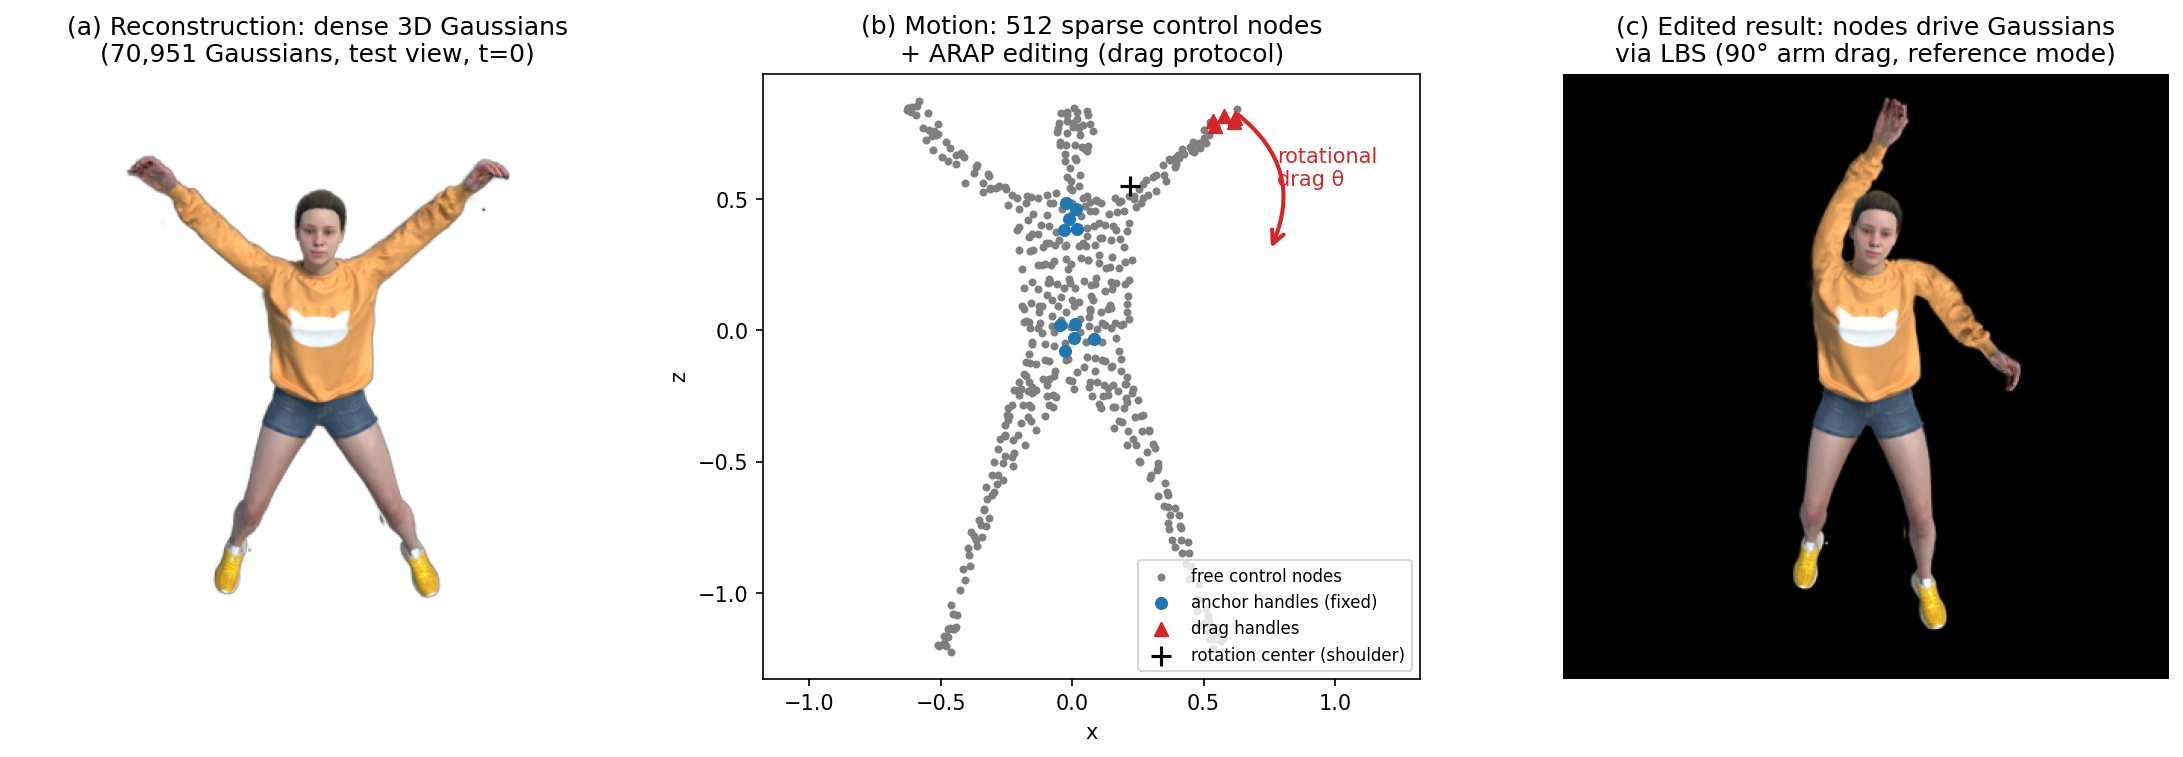
\includegraphics[width=0.90\textwidth]{method_overview.png}
  \caption{\textbf{SC-GS at a glance.} (a)~Dense canonical Gaussians carry
  appearance (\texttt{jumpingjacks}, 70{,}951 Gaussians). (b)~512 sparse
  control nodes carry motion; editing constrains a drag-handle group (red, here
  rotated about the shoulder along an arc) and anchor groups (blue), and solves
  ARAP for all remaining nodes. (c)~The solved node field drives the Gaussians
  through LBS.}
  \label{fig:overview}
\end{figure*}

SC-GS represents a dynamic scene as canonical 3DGS parameters plus $M$ control
nodes ($M{=}512$ by default) with learned radii. A deformation MLP maps
$(\mathbf{p}_i, t)$ to per-node translation; each Gaussian is skinned to its
$K$ nearest nodes with Gaussian-kernel LBS weights, and an ARAP-style
regularizer on sampled node trajectories biases training toward locally rigid
motion (Fig.~\ref{fig:overview}). File/line references below are to the
official implementation.

\paragraph{Editing}
At edit time $t$, node positions $\mathbf{p} = \mathrm{nodes} + d_{xyz}(t)$
form a graph with trajectory-aware connectivity ($K{=}16$). The user selects a
\emph{handle} group (a clicked node plus its 2-ring) and drags it; anchors are
additional handle groups with zero displacement. Writing $\mathcal{E}$ for the
graph edges with weights $w_{ij}$, the solver
(\texttt{utils/arap\_deform.py:86}) minimizes the ARAP energy
\begin{equation}
  E(\mathbf{p}') \;=\; \sum_{(i,j)\in\mathcal{E}} w_{ij}
  \bigl\lVert (\mathbf{p}'_i - \mathbf{p}'_j) -
  \mathbf{R}_i (\mathbf{p}_i - \mathbf{p}_j) \bigr\rVert^2 ,
  \label{eq:arap}
\end{equation}
subject to hard handle constraints, by local-global iteration --- per-node SVD
fitting of $\mathbf{R}_i$ alternating with a linear solve for $\mathbf{p}'$
--- but runs only $\mathrm{NUM\_ITER}=3$ iterations per call. Two GUI modes
differ \emph{only in initialization} (\texttt{train\_gui.py:768--777}):
\begin{itemize}\itemsep1pt
  \item \fromInit{} (default; hereafter ``\textbf{\scgsOrig{}}'', the baseline
        our method improves upon): every solve starts from the linear
        Laplacian-editing least-squares solution
        $\mathbf{p}'^{(0)} = \arg\min_{\mathbf{p}'}
        \lVert \mathbf{L}\mathbf{p}' - \mathbf{L}\mathbf{p} \rVert^2$
        s.t.\ handles (\texttt{arap\_deform.py:103});
  \item \iterMode{} (hereafter ``\textbf{\scgsIter{}}''): every solve
        warm-starts from the previous drag event's solution
        (\texttt{init\_verts}); robust but ${\sim}100\times$ slower over a
        large drag, and stateful. We use it as the robustness
        \emph{reference}, not as a practical competitor.
\end{itemize}

\paragraph{Propagation}
The solved node displacement field is not paired with the solver's rotations.
Instead, node rotations are re-estimated from the displaced node positions by a
local SVD fit (\texttt{p2dR}, \texttt{time\_utils.py:1044}), and Gaussians are
re-expressed relative to their deformed neighbor nodes with these rotations
(\texttt{time\_utils.py:1196--1213}). Consequently, any non-rigidity in the
node field converts directly into inconsistent rotations and stretched Gaussian
layouts.

% =====================================================================
\section{An Empirical Study of Editing Failures}
\label{sec:failures}

\subsection{Methodology}
\label{sec:method-study}

We script the GUI pipeline headlessly and call-for-call (animation
initialization $\rightarrow$ keypoint selection with $n$-ring expansion
$\rightarrow$ \texttt{deform\_arap} $\rightarrow$
\texttt{deform.step(node\_trans\_bias)} $\rightarrow$ render), so that measured
behavior is exactly the interactive system's. The canonical protocol drags a
limb-tip handle group (nearest node + 1-ring) along the arc of a joint rotation
--- \eg{} the \texttt{jumpingjacks} hand rotated about the shoulder in the
frontal plane --- with the torso held by two anchor groups; intermediate limb
nodes are free, so the solver must infer the limb's rotation. Handle
constraints are hard and both modes satisfy them exactly (residual 0): all
differences live in the free nodes. The \iterMode{} mode applied in
1$^\circ$ warm-started sub-steps serves as the \emph{reference} (it emulates
GUI mouse granularity); a single \fromInit{} solve at angle $\theta$ is exactly
the state the default mode reaches at accumulated angle $\theta$, since that
mode re-solves from scratch at the current absolute targets on every drag
event.

Per angle $\theta \in [5^\circ, 135^\circ]$ we measure:
\begin{itemize}\itemsep1pt
  \item \textbf{Graph rigidity}: relative edge-length distortion over the ARAP
        graph (mean/p95/max, globally and in the drag region = handle + 4
        rings) and the ARAP energy of Eq.~\eqref{eq:arap} between rest and
        deformed nodes;
  \item \textbf{Gaussian-level tearing}: p95 of per-Gaussian maximum
        neighbor-distance stretch ($K{=}8$ canonical neighbors) in the edited
        region, after LBS propagation;
  \item \textbf{Off-region leakage}: p95 displacement of nodes \emph{outside}
        the drag region and anchors --- a global metric designed to expose
        smooth drift that edge-based statistics cannot see
        (\S\ref{sec:failureB});
  \item \textbf{Image deviation}: PSNR/SSIM/LPIPS~\cite{lpips} of the rendered
        edit against the reference mode's render at the same $\theta$ and
        camera;
  \item \textbf{Latency}: wall-clock solve time (GPU-synced).
\end{itemize}
All protocol constants (seed points, rotation centers, axes, cameras) are
serialized to JSON alongside the committed metric CSVs.

\subsection{Failure I: rotation-blind initialization under large rotational drags}
\label{sec:failureA}

\begin{figure*}[t]
  \centering
  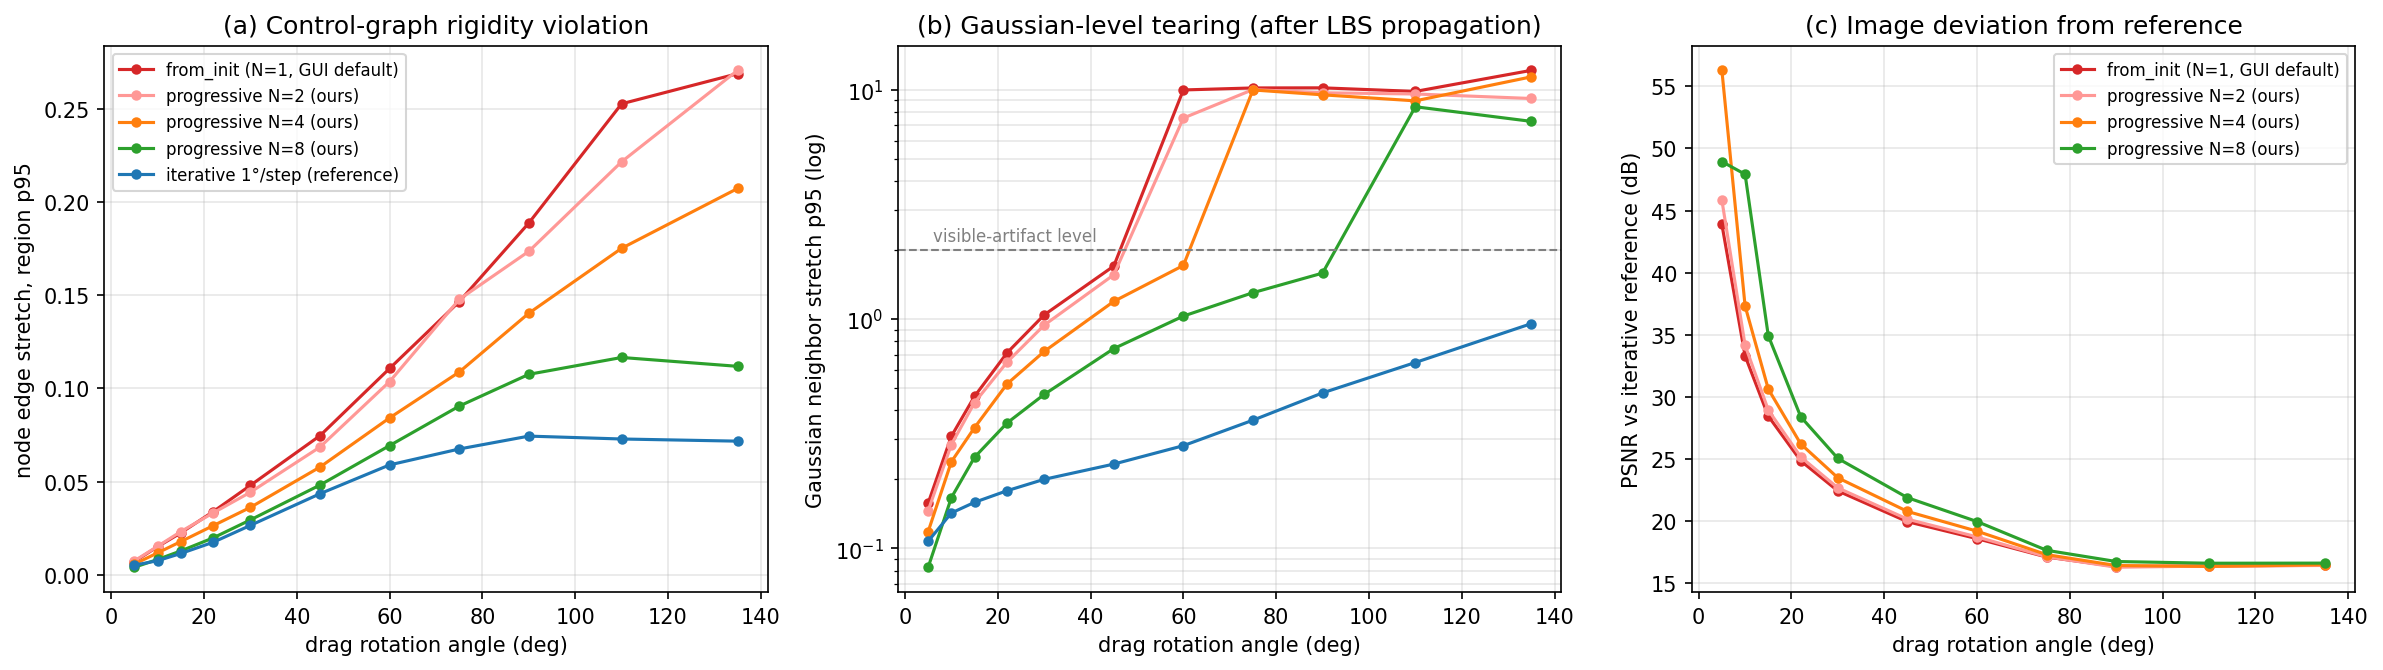
\includegraphics[width=0.95\textwidth]{failureA_curves.png}
  \caption{\textbf{Original SC-GS vs.\ our method under shoulder-rotation
  drags} (\texttt{jumpingjacks}). (a)~Node-graph rigidity violation vs.\ drag
  angle. (b)~Gaussian-level tearing after LBS propagation (log scale); the
  dashed line marks the level at which artifacts are clearly visible.
  (c)~Image deviation from the reference. \scgsOrig{} (red) departs from the
  slow reference (blue) between 45$^\circ$ and 60$^\circ$; our progressive
  schedules (pink/orange/green, \S\ref{sec:method}) recover monotonically
  toward the reference as $N$ grows, at a fraction of its cost.}
  \label{fig:failureA}
\end{figure*}

Fig.~\ref{fig:failureA} quantifies the failure on \texttt{jumpingjacks}. The
default mode tracks the reference up to ${\sim}30^\circ$, then departs sharply:
across $45^\circ{\rightarrow}60^\circ$ its Gaussian-stretch statistic jumps
$1.70 \rightarrow 9.98$ while the reference stays below $0.3$ --- a six-fold
discontinuity that localizes the \textbf{failure onset to 45--60$^\circ$}. At
135$^\circ$ the node edge stretch reaches $3.8\times$ the reference (0.269 vs.\
0.072) and the ARAP energy is doubled (0.093 vs.\ 0.048). Visually
(Fig.~\ref{fig:qualitative}, top row) the limb \emph{under-rotates} --- at
90--135$^\circ$ the arm remains near-horizontal instead of following the arc
--- \emph{shortens} toward the chord, and the hand \emph{shreds} into a blob of
disconnected Gaussians.

The mechanism follows \S\ref{sec:prelim}: the Laplacian initialization is a
linear solve that cannot represent rotation~\cite{lse,botsch}; for a rotational
drag it produces the chord-shortcut configuration, and three local-global
iterations --- each of which only re-estimates local rotations from the
\emph{current} guess --- make insufficient progress from so poor a start. The
reference mode avoids this entirely because its per-event increments
(${\sim}1^\circ$) keep every solve within the basin that three iterations can
handle. Robustness, however, costs latency: the accumulated reference solves
for a 135$^\circ$ drag take 12.3\,s versus 0.11\,s for the one-shot default ---
a 100$\times$ gap that explains why the fast mode is the GUI default.

\subsection{Failure II: propagation-stage rotation re-estimation}
\label{sec:failureII}

A control experiment isolates a second, initialization-independent artifact.
When the \emph{entire} handle group is rotated about its own centroid (the
GUI's rotation-drag semantics, leaving no free nodes inside the moved region),
both modes produce near-identical node fields --- yet \textbf{both} shred the
limb beyond ${\sim}75^\circ$ (Gaussian stretch p95 $\approx$ 8--12). The blame
therefore lies downstream of the ARAP solve: the \texttt{p2dR} stage
re-estimates node rotations from displaced positions and blends Gaussians
across the handle boundary with Floyd-graph LBS weights; under a large in-place
rotation of a small node cluster, boundary Gaussians receive inconsistent
rotation estimates and tear. This artifact is orthogonal to initialization and
is \emph{not} repaired by our method (\S\ref{sec:discussion}); we report it as
a distinct failure axis.

\subsection{Failure III: sensitivity to control-point count}
\label{sec:failureB}

\begin{figure*}[t]
  \centering
  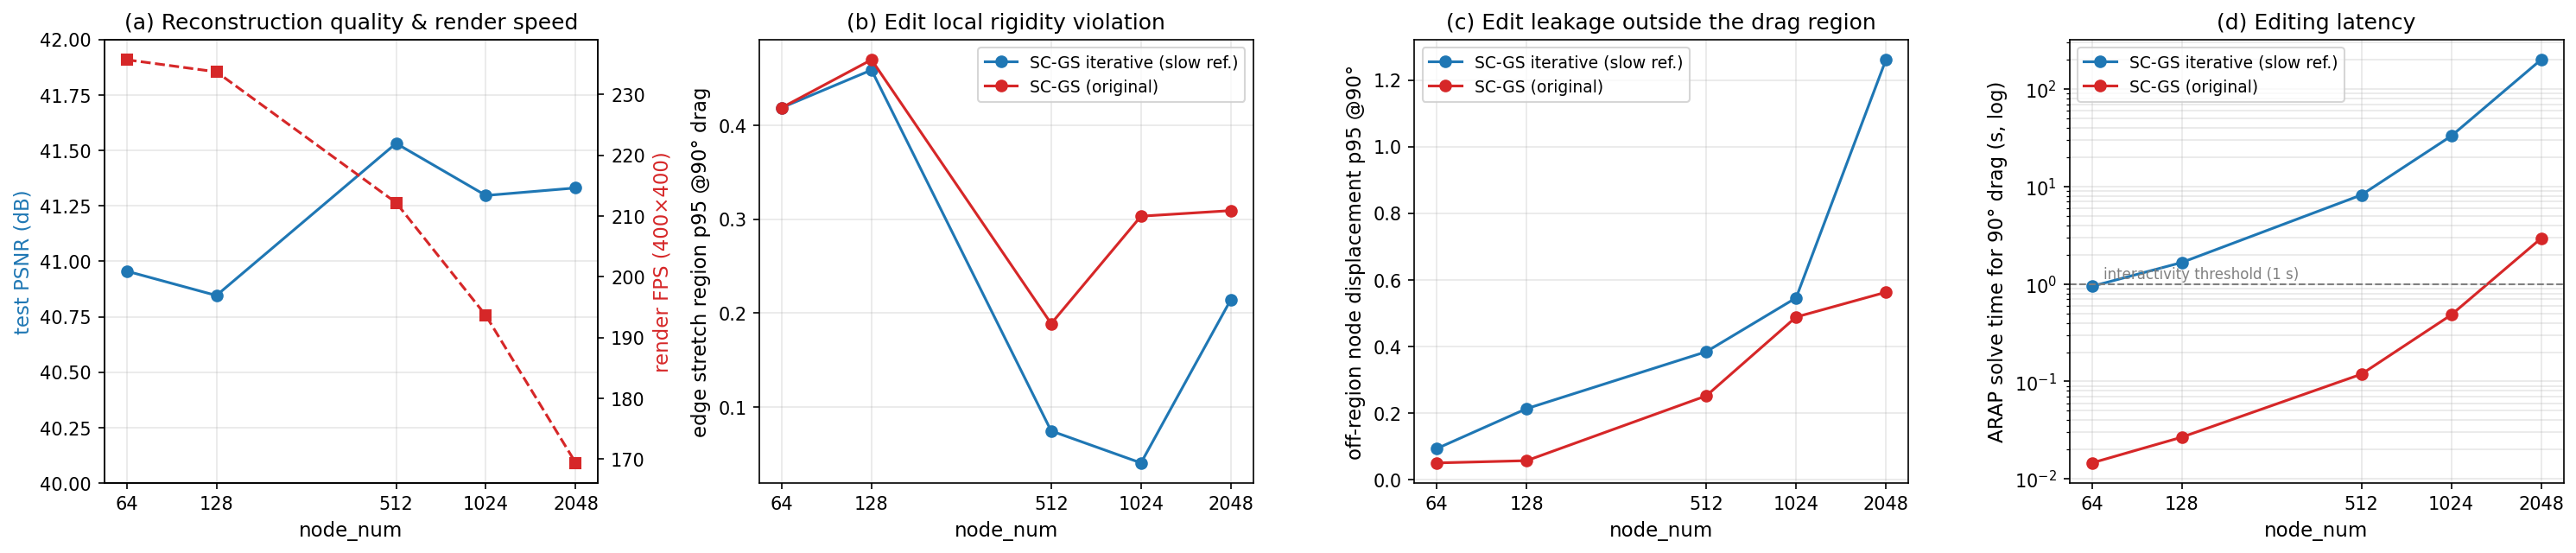
\includegraphics[width=0.95\textwidth]{failureB_curves.png}
  \caption{\textbf{Control-point count sweep on \texttt{jumpingjacks}}
  ($M \in \{64, 128, 512, 1024, 2048\}$, identical training). (a)~Test PSNR is
  flat while render FPS falls 28\%. (b)~Edit rigidity is U-shaped.
  (c)~Off-region leakage grows monotonically with node count and is worst for
  the warm-started mode. (d)~Solve latency crosses the interactivity
  threshold.}
  \label{fig:failureB}
\end{figure*}

\begin{table*}[t]
  \centering\small
  \caption{\textbf{Control-point sweep} (\texttt{jumpingjacks};
  \S\ref{sec:failureB}). ``ref'' = \iterMode{}, ``def'' = \fromInit{}.}
  \label{tab:nodesweep}
  \begin{tabular}{lccccc}
    \toprule
    node count $M$ & 64 & 128 & 512 & 1024 & 2048 \\
    \midrule
    test PSNR (dB) & 40.96 & 40.85 & \textbf{41.53} & 41.30 & 41.33 \\
    render FPS ($400^2$) & 235.7 & 233.7 & 212.2 & 193.6 & 169.4 \\
    edge stretch p95 @90$^\circ$ (ref / def) & 0.42 / 0.42 & 0.46 / 0.47 & 0.07 / 0.19 & 0.04 / 0.30 & 0.21 / 0.31 \\
    leakage p95 @90$^\circ$ (ref / def) & 0.09 / 0.05 & 0.21 / 0.06 & 0.38 / 0.25 & 0.55 / 0.49 & \textbf{1.26} / 0.56 \\
    solve time @90$^\circ$ (ref / def) & 0.9 / 0.01\,s & 1.7 / 0.03\,s & 8.2 / 0.12\,s & 33 / 0.48\,s & 200 / 2.9\,s \\
    \bottomrule
  \end{tabular}
\end{table*}

Retraining \texttt{jumpingjacks} across a 32$\times$ range of control-point
counts (Tab.~\ref{tab:nodesweep}, Fig.~\ref{fig:failureB}) shows that
\textbf{novel-view quality is essentially independent of node count} (spread
0.7\,dB; the default 512 is best) --- in this regime node count is an
\emph{editability and cost} knob, not a quality knob. Editing, by contrast,
fails at both extremes:
\begin{itemize}\itemsep2pt
  \item \textbf{Low extreme (64--128 nodes): articulation failure.} Under the
        standard 90$^\circ$ drag both solver modes produce nearly identical,
        heavily distorted results (region edge stretch 0.42--0.47, six times
        the 512-node reference); the limb cannot bend at the joint because
        deformation granularity is bounded by node spacing. The failure is
        solver-independent.
  \item \textbf{High extreme (2048 nodes): latency and leakage failure.} A
        single default-mode solve takes 3.0\,s (25$\times$ the 512-node cost)
        and the 90$^\circ$ reference drag takes 200\,s. More insidiously, the
        reference mode rips \emph{off-region} geometry: p95 off-region node
        displacement reaches \textbf{1.26 scene units} (body height
        ${\approx}2$) --- the character's legs are visibly torn sideways by an
        arm drag --- while every \emph{local} rigidity statistic stays
        moderate, because the drift is spatially smooth. This is precisely why
        we introduce the leakage metric. Leakage grows monotonically with node
        count (reference @90$^\circ$: $0.09 \rightarrow 0.21 \rightarrow 0.38
        \rightarrow 0.55 \rightarrow 1.26$) and is ${\sim}2\times$ worse for
        the warm-started reference than for the stateless default at 2048
        nodes: warm-start drift \emph{accumulates} across the 90 sub-steps.
        \textbf{The preferable solver mode therefore inverts at the high
        extreme} --- the mode that repairs Failure~I is the one that fails
        here.
\end{itemize}

% =====================================================================
\section{Method: Progressive Drag Scheduling}
\label{sec:method}

\begin{figure*}[t]
  \centering
  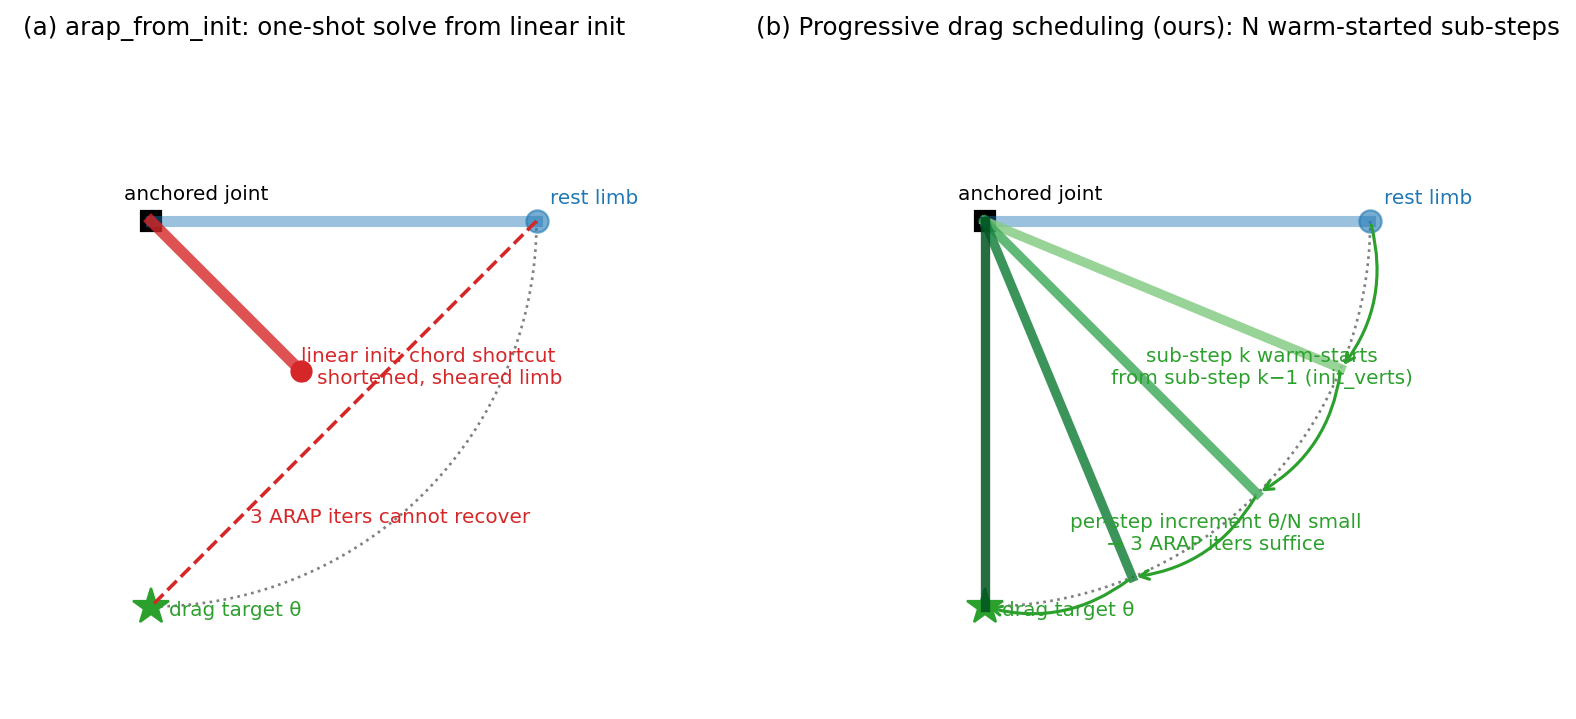
\includegraphics[width=0.82\textwidth]{fig_method_schematic.png}
  \caption{\textbf{Why one-shot solves fail and progressive scheduling repairs
  them.} (a)~The linear initialization moves free nodes along the chord toward
  the target, shortening and shearing the limb; three ARAP iterations cannot
  climb back to the arc. (b)~Subdividing the drag into $N$ sub-targets along
  the arc keeps every increment small; each solve warm-starts from the previous
  solution, so three iterations per sub-step suffice.}
  \label{fig:schematic}
\end{figure*}

Failure~I is caused by the conjunction of a rotation-blind initializer and a
hard iteration budget. Rather than modifying either (retraining nothing,
touching no solver code), we change \emph{what the solver is asked to do}.
Given rest handle positions $H_0$, final targets $H(\theta)$ obtained by
rotating the handle group about a drag center $\mathbf{c}$ with axis
$\mathbf{a}$, and a schedule length $N$:
\begin{equation}
  H_k \;=\; H\!\left(\tfrac{k}{N}\,\theta\right),\qquad
  \mathbf{p}'^{(k)} \;=\; \mathrm{ARAP}_3\!\left(H_k;\;
  \mathrm{init} = \mathbf{p}'^{(k-1)}\right),
  \label{eq:schedule}
\end{equation}
for $k = 1,\dots,N$, where $\mathrm{ARAP}_3$ denotes the stock three-iteration
solver and $\mathbf{p}'^{(0)}$ is the Laplacian initialization (harmless at
small angles). Algorithm~\ref{alg:pds} summarizes the procedure.

\begin{algorithm}[t]
\caption{Progressive Drag Scheduling}
\label{alg:pds}
\begin{algorithmic}[1]
\Require rest nodes $\mathbf{p}$, handle set $\mathcal{H}$, targets $H(\theta)$, steps $N$
\State $\mathbf{p}' \gets \textsc{nil}$ \Comment{first step: Laplacian init}
\For{$k = 1$ \textbf{to} $N$}
  \State $H_k \gets H(\theta k / N)$ \Comment{slerp about drag center}
  \State $\mathbf{p}' \gets \Call{DeformARAP}{\mathcal{H},\, H_k,\, \mathrm{init\_verts}=\mathbf{p}'}$
\EndFor
\State \Return node displacement field $\mathbf{p}' - \mathbf{p}$
\end{algorithmic}
\end{algorithm}

The result is a deterministic function of (rest state, final targets, $N$) ---
unlike the reference mode it does not depend on the user's drag history, can be
re-executed from a stored keyframe, and has bounded latency $N \cdot
t_{\mathrm{solve}}$. Conceptually, the schedule replaces one hopeless global
solve by $N$ easy local ones: each sub-step's increment $\theta/N$ stays within
the basin in which three local-global iterations converge, and the warm start
transports the solution along the arc (Fig.~\ref{fig:schematic}). Setting
$N{=}1$ recovers \fromInit{}; $N \rightarrow \theta/1^\circ$ recovers the
reference. In our implementation the schedule lives entirely in the editing
driver: each sub-step reuses the exact \texttt{deform\_arap(init\_verts=$\cdot$)}
call the GUI already issues for its iterative mode, so a GUI integration is a
${\sim}$10-line loop.

% =====================================================================
\section{Experiments}
\label{sec:experiments}

\subsection{Execution environment and reproduction}
\label{sec:setup}

All experiments use the official SC-GS implementation (fixed seed, 80k
iterations, $400\times400$ --- the D-NeRF comparison convention) on a Quadro
RTX~5000; environment and build details, including a gcc-13 compilation fix,
are documented in the repository. Tab.~\ref{tab:repro} verifies that our
trained models reproduce the paper.

\begin{table*}[t]
  \centering\small
  \caption{\textbf{Reproduction on D-NeRF} (test split). Paper numbers from
  SC-GS Tab.~1~\cite{scgs}. $^{*}$Gaps beyond 0.5\,dB, investigated:
  \texttt{trex} --- best checkpoint during training reached 40.86
  (${\approx}0.2$\,dB is final-iteration checkpoint selection), SSIM matches
  and LPIPS is better than the paper's; the finest structures in the benchmark,
  residual consistent with densification variance. \texttt{bouncingballs} ---
  best checkpoint 42.61, LPIPS again better than the paper's (.0142 vs .0166);
  the scene is dominated by large smooth motions where PSNR is highly sensitive
  to sub-pixel phase. $^{\dagger}$SC-GS does not report \texttt{lego} (its
  D-NeRF test split is known to be misaligned); we train it only as an editing
  test bed (mechanical joint).}
  \label{tab:repro}
  \setlength{\tabcolsep}{4.5pt}
  \begin{tabular}{lccccc}
    \toprule
    Scene & PSNR paper / ours ($\Delta$) & SSIM paper / ours & LPIPS paper / ours & Train & Peak GPU \\
    \midrule
    jumpingjacks & 41.13 / \textbf{41.53} ($+0.40$) & .998 / .9975 & .0067 / .0058 & 64.9\,min & 1.47\,GiB \\
    hook         & 39.87 / 39.74 ($-0.13$)          & .997 / .9963 & .0076 / .0084 & 65.4\,min & 1.91\,GiB \\
    mutant       & 45.19 / 45.03 ($-0.16$)          & .999 / .9990 & .0028 / .0029 & 63.5\,min & 2.08\,GiB \\
    standup      & 47.89 / 47.51 ($-0.38$)          & .999 / .9991 & .0023 / .0025 & 65.5\,min & 3.02\,GiB \\
    trex         & 41.24 / 40.68 ($-0.56$)$^{*}$    & .998 / .9985 & .0046 / .0038 & 65.6\,min & 2.07\,GiB \\
    hellwarrior  & 42.93 / \textbf{43.00} ($+0.07$) & .994 / .9931 & .0155 / .0165 & 63.7\,min & 1.33\,GiB \\
    bouncingballs& 44.91 / 42.55 ($-2.36$)$^{*}$    & .998 / .9966 & .0166 / .0142 & 68.3\,min & 3.74\,GiB \\
    lego$^{\dagger}$ & --- / 25.36                  & --- / .9481  & --- / .0386   & 63.6\,min & 1.30\,GiB \\
    \bottomrule
  \end{tabular}
\end{table*}

\subsection{Main results}
\label{sec:main}

\begin{figure*}[t]
  \centering
  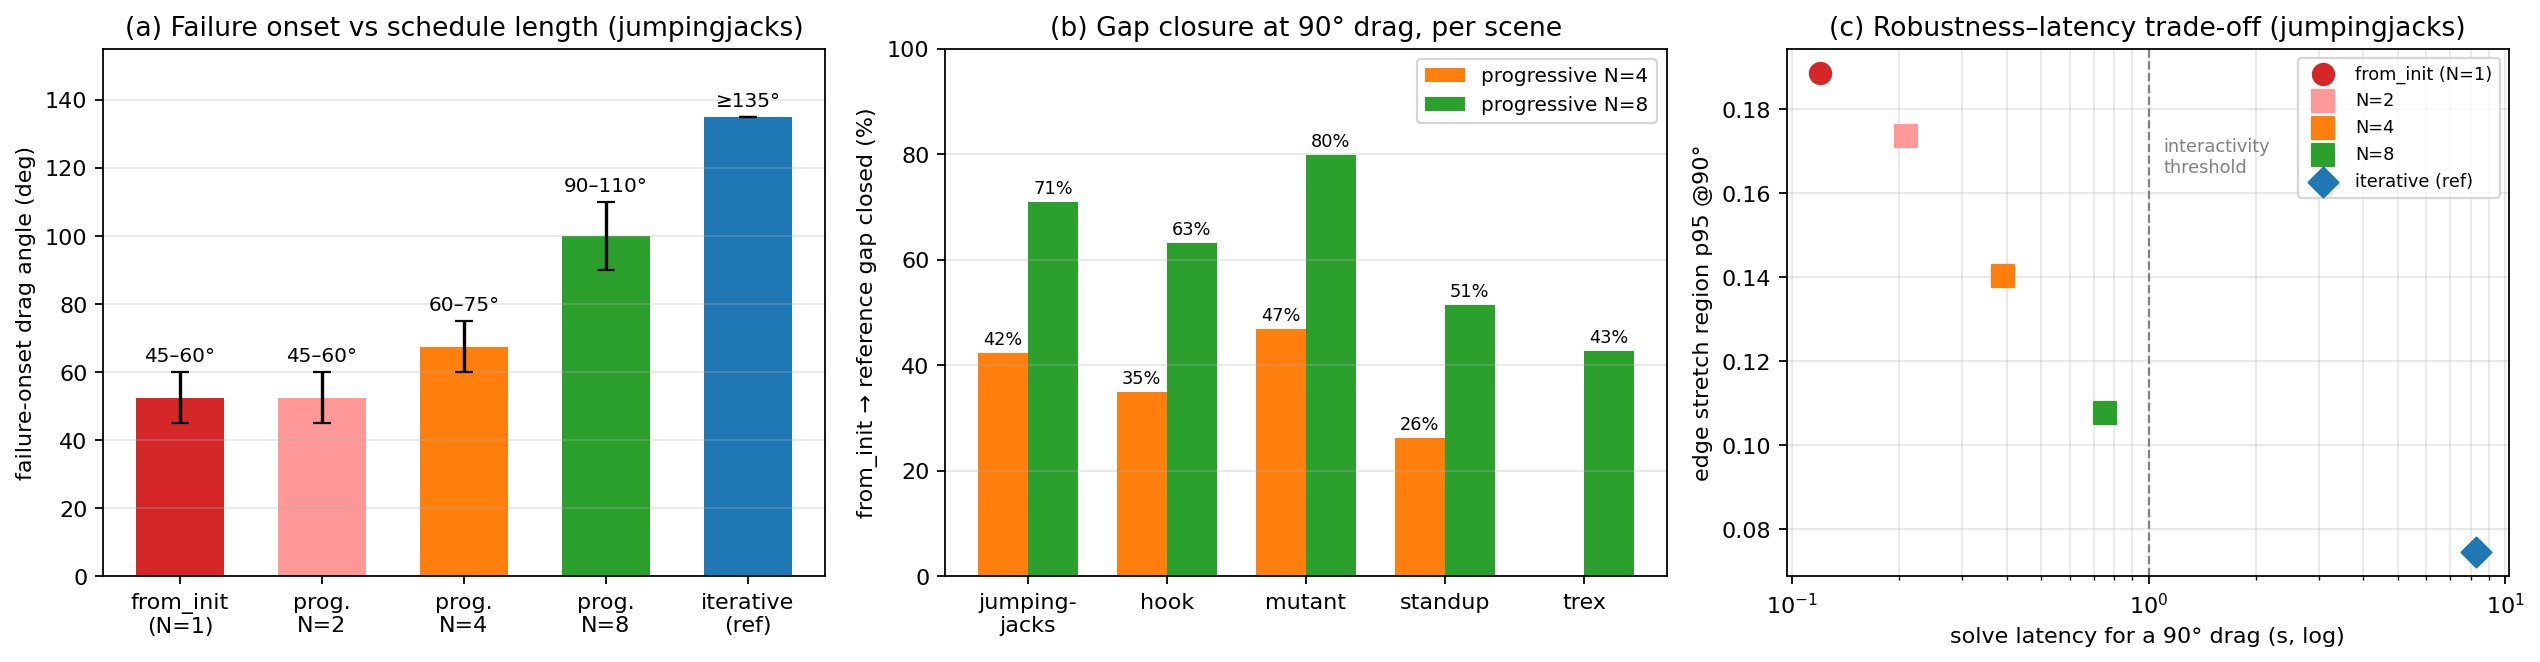
\includegraphics[width=0.95\textwidth]{fig_onset_gapclosure.png}
  \caption{\textbf{How far our method moves SC-GS toward its robustness upper
  bound.} (a)~Failure-onset angle grows with schedule length $N$: from
  45--60$^\circ$ for \scgsOrig{} to 90--110$^\circ$ for \ours{8} (bars: onset
  interval from the angle sweep). (b)~Fraction of the
  original$\rightarrow$reference rigidity gap closed by our method at a
  90$^\circ$ drag, per scene (edge-stretch region p95; \texttt{trex} $N{=}4$
  closes 0\% on this node-level metric --- but see \S\ref{sec:hardcase} and
  the image-level metrics). (c)~The robustness--latency plane at 90$^\circ$:
  our schedules populate the previously empty region between the two original
  SC-GS modes, below the 1\,s interactivity threshold.}
  \label{fig:onset}
\end{figure*}

\begin{table}[t]
  \centering\small
  \caption{\textbf{Failure onset and cost} (\texttt{jumpingjacks}). Onset =
  first angle at which Gaussian stretch p95 exceeds the visible-artifact level
  (${\approx}2$).}
  \label{tab:onset}
  \setlength{\tabcolsep}{4pt}
  \begin{tabular}{lcccc}
    \toprule
    mode & onset & \begin{tabular}{@{}c@{}}edge p95\\@135$^\circ$\end{tabular} &
    \begin{tabular}{@{}c@{}}ARAP\\@135$^\circ$\end{tabular} &
    \begin{tabular}{@{}c@{}}solve\\@135$^\circ$\end{tabular} \\
    \midrule
    \scgsOrig{}          & 45--60$^\circ$ & 0.269 & 0.093 & 0.11\,s \\
    \ours{2}             & 45--60$^\circ$ & 0.271 & 0.091 & 0.21\,s \\
    \ours{4}             & 60--75$^\circ$ & 0.207 & 0.073 & 0.39\,s \\
    \ours{8}             & \textbf{90--110$^\circ$} & 0.112 & 0.051 & 0.76\,s \\
    \scgsIter{} (slow ref.) & $\geq$135$^\circ$ & 0.072 & 0.048 & 12.34\,s \\
    \bottomrule
  \end{tabular}
\end{table}

Robustness scales monotonically with $N$ (Tab.~\ref{tab:onset},
Fig.~\ref{fig:failureA}): $N{=}8$ covers the practical editing range
($\leq$90$^\circ$) at $\leq$0.8\,s per drag --- 16$\times$ cheaper than the
reference at 135$^\circ$ --- and every image metric against the reference
improves monotonically in $N$ at every angle (\eg{} PSNR at 60$^\circ$:
$18.59 \rightarrow 19.97$\,dB; LPIPS at 45$^\circ$: $0.097 \rightarrow 0.066$).
Beyond its onset, each schedule fails exactly like the default mode --- the
\emph{final} sub-step's increment exceeds what three iterations absorb ---
implying that $N$ should scale with $\theta$; the onset table yields the simple
adaptive rule $N = \lceil \theta / 15^\circ \rceil$ (fix the per-substep
increment at 10--15$^\circ$).

\begin{figure}[!htb]
  \centering
  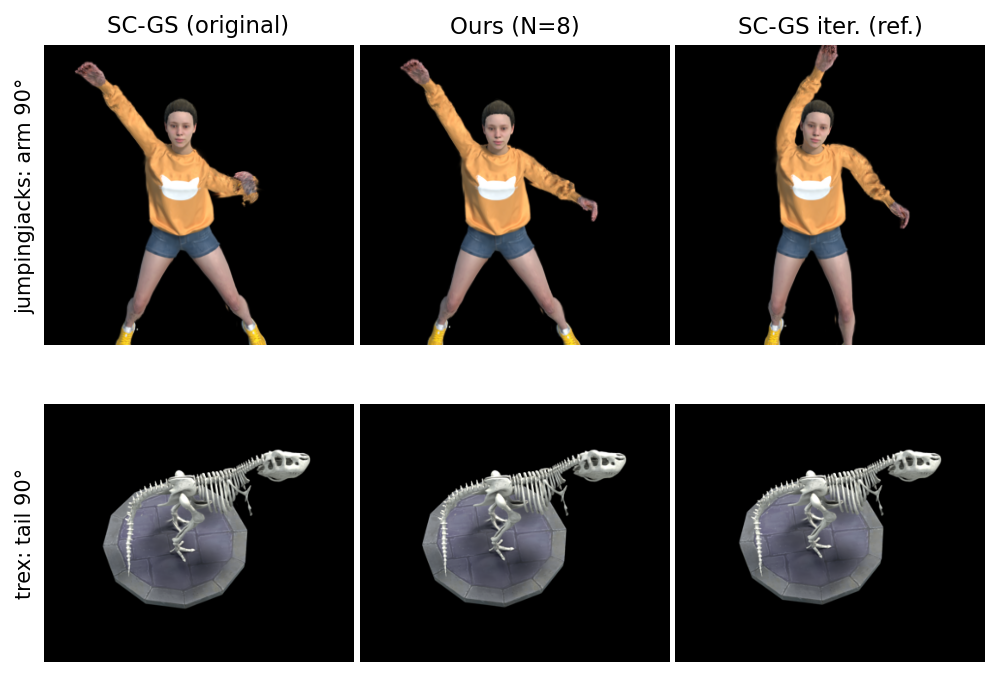
\includegraphics[width=\linewidth]{fig_qualitative_2scene.png}
  \caption{\textbf{Original SC-GS vs.\ our method at a 90$^\circ$ drag} on the
  easiest-to-see cases. Top: \texttt{jumpingjacks} --- the original mode leaves
  the arm near-horizontal with a shredded hand; ours restores the intended
  lowered pose. Bottom: \texttt{trex} --- the original mode shortens and kinks
  the tail; ours restores the smooth arc. Per-angle grids for all eight scenes
  are in the repository.}
  \label{fig:qualitative}
\end{figure}

\subsection{Cross-scene generalization}
\label{sec:crossscene}

\begin{table*}[t]
  \centering\small
  \caption{\textbf{Original SC-GS vs.\ our method across eight scenes: node
  edge stretch (region p95) at 90$^\circ$ / 135$^\circ$.} Lower is better; the
  reference mode is the robustness upper bound at ${\sim}100\times$ the
  latency. Our schedules improve on the original monotonically in $N$ on every
  scene (two isolated exceptions: \texttt{trex} $N{=}2$ and
  \texttt{bouncingballs} $N{=}8$@90$^\circ$, both within metric noise).}
  \label{tab:crossscene}
  \scriptsize
  \setlength{\tabcolsep}{2.6pt}
  \begin{tabular}{lcccccccc}
    \toprule
    mode & jump.jacks & hook & mutant & standup & trex & hellwarr. & lego & bounc.balls \\
    \midrule
    \scgsOrig{}          & .189/.269 & .213/.318 & .237/.399 & .362/.439 & .285/.410 & .192/.307 & .420/.623 & .216/.350 \\
    \ours{2}             & .174/.271 & .201/.285 & .211/.337 & .344/.409 & .295/.421 & .182/.268 & .391/.580 & .198/.279 \\
    \ours{4}             & .140/.207 & .169/.228 & .177/.258 & .310/.389 & .285/.391 & .142/.211 & .371/.548 & .155/.202 \\
    \ours{8}             & .108/.112 & .134/.175 & .135/.221 & .261/.307 & .267/.371 & .113/.166 & .358/.515 & .172/.200 \\
    \scgsIter{} (slow ref.) & .074/.072 & .088/.125 & .109/.157 & .165/.181 & .244/.342 & .092/.139 & .328/.402 & .155/.183 \\
    \bottomrule
  \end{tabular}
\end{table*}



We repeat the full protocol (5 modes $\times$ 11 angles) on seven additional
scenes covering qualitatively different articulation types: organic limbs
(\texttt{hook} forward arm / axis $X$; \texttt{mutant} claw arm / $Y$;
\texttt{standup} crouched forward arm / $X$; \texttt{hellwarrior} spread arm /
$Y$), an extreme kinematic chain (\texttt{trex} tail about its root / $Z$), a
\emph{mechanical} joint (\texttt{lego} bulldozer shovel about its hinge / $X$),
and an unarticulated free body (\texttt{bouncingballs}: a ball dragged along an
arc above the plate / $Y$ --- included to test whether the failure requires an
articulated chain at all; it does not, since the arc drag alone triggers the
chord-shortcut init). The ordering \scgsOrig{} $>$ \ours{2} $>$ \ours{4} $>$
\ours{8} $>$ reference is \textbf{monotone at every tested angle on six of the
eight scenes}, with two isolated single-point exceptions within metric noise
(Tab.~\ref{tab:crossscene}; per-scene curves for all
eight scenes are in the repository). At 90$^\circ$ \ours{8}
closes 43--80\% of the original$\rightarrow$reference gap: 71\%
(\texttt{jumpingjacks}), 63\% (\texttt{hook}), 80\% (\texttt{mutant}), 51\%
(\texttt{standup}), 43\% (\texttt{trex}), 79\% (\texttt{hellwarrior}), 67\%
(\texttt{lego}), 72\% (\texttt{bouncingballs}) (Fig.~\ref{fig:onset}b), and
image deviation from the reference improves monotonically in $N$ on all eight
scenes (\eg{} PSNR at 90$^\circ$: \texttt{hellwarrior} $34.0 \rightarrow
36.4$\,dB, \texttt{lego} $18.6 \rightarrow 21.1$\,dB, \texttt{bouncingballs}
$20.2 \rightarrow 21.9$\,dB from \scgsOrig{} to \ours{8}). Artifact
\emph{severity} varies with limb geometry --- Gaussian stretch p95 at
90$^\circ$ is 10.2 on \texttt{jumpingjacks}' thin arm but only 1.6 on
\texttt{mutant}'s thick claw --- yet the qualitative conclusion is unchanged
everywhere.

\subsection{The hard case: \texttt{trex}}
\label{sec:hardcase}

The \texttt{trex} tail is a single long elastic chain far from every anchor,
and it stresses every mode: even the reference reaches 0.34 edge stretch at
135$^\circ$. Node-level differences between modes compress
(Tab.~\ref{tab:crossscene}), and \ours{2} is statistically indistinguishable
from the original --- its 45--67$^\circ$ sub-steps already exceed the per-step
failure level, so warm-starting buys nothing. Yet the \emph{visual} verdict is
unambiguous (Fig.~\ref{fig:qualitative}, bottom row): the original mode's tail
is visibly shortened and kinked, while \ours{4}/\ours{8} restore the smooth
arc; image metrics agree (PSNR vs.\ reference at 90$^\circ$: $24.7
\rightarrow 25.0 \rightarrow 27.7$\,dB from original to $N{=}4$ to $N{=}8$;
LPIPS $0.039 \rightarrow 0.018$). The \texttt{lego} hinge is the
second-hardest case for the same reason in a mechanical guise --- rigid
brick blocks tolerate no distortion at all, so every mode carries high
absolute error, yet the ordering and the monotone image-level recovery are
identical. We draw two honest conclusions: progressive scheduling helps on
every scene we tested, but it is not a silver bullet for extreme kinematic
chains; and geometry-level and image-level metrics can dissociate ---
evaluations relying on a single family of metrics would have mis-ranked these
cases in both directions.

% =====================================================================
\section{Discussion and Limitations}
\label{sec:discussion}

\paragraph{A robustness--latency--statefulness triangle}
Our analysis reframes SC-GS's two editing modes as corners of a design
triangle: the default mode is fast, deterministic, and restorable but
rotation-blind; the reference mode is robust to rotation but slow, stateful,
and --- at high control-point counts --- the more dangerous mode due to drift
accumulation (\S\ref{sec:failureB}). Progressive scheduling occupies the useful
interior: bounded latency, deterministic output, and a robustness dial.
Fig.~\ref{fig:onset}c makes the geometry of this trade-off explicit.

\paragraph{What benchmarks do not measure}
Reconstruction quality was flat across every intervention that dramatically
changed editability (Tab.~\ref{tab:nodesweep}). For editable representations,
we argue evaluation should include editing-stress protocols of the kind
proposed here --- angle sweeps with rigidity, leakage, and reference-deviation
metrics --- rather than novel-view metrics alone.

\paragraph{Limitations}
(i)~Our improvement addresses the initialization failure only; the
propagation-stage artifact (\S\ref{sec:failureII}) and the high-count leakage
failure (\S\ref{sec:failureB}) are orthogonal and unrepaired --- at
$\geq$110$^\circ$ even $N{=}8$ fails, and on \texttt{trex} the reference itself
is stressed. Blending the ARAP solver's own rotations instead of re-estimating
them from positions, and anchoring or damping the global solve against
off-region drift, are natural next steps. (ii)~The iteration budget
$\mathrm{NUM\_ITER}=3$ was deliberately held fixed to isolate the scheduling
effect; jointly scheduling sub-steps and iterations (\eg{} extra iterations on
the final sub-step) is unexplored. (iii)~One drag protocol per scene, with
seeds chosen once and documented; a user study or randomized-protocol sweep
would strengthen external validity. (iv)~The reference mode is a strong
baseline, not ground truth --- it drifts at extreme angles and leaks at high
node counts.

\paragraph{Reproducibility}
Every experiment derives from a committed artifact: one script per experiment,
29 dated entries in an experiment log, metric CSVs and figures under
\texttt{results/}, and per-protocol JSON seed files (drag points, anchors,
rotation centers/axes, cameras). Each figure and table here is regenerated by a
single documented command (repository README). Training uses the upstream fixed
seed; residual nondeterminism is limited to rasterizer atomics during
densification.

\paragraph{Use of generative AI}
Claude Code (Anthropic Fable~5) was used as a research-engineering assistant
for environment setup, code reading, experiment scripting and execution, figure
generation, and draft text; the running log of tools, purposes, and
human-revised parts is \texttt{docs/AI\_USAGE\_LOG.md} in the repository. All
quantitative claims are machine-generated from the committed measurement CSVs
rather than written by hand, and all protocol choices are serialized alongside
the results. The author reviewed and revised the content and is responsible for
it.

% =====================================================================
\section{Conclusion}
\label{sec:conclusion}

We presented a systematic failure analysis of the SC-GS editing pipeline,
localizing a sharp large-rotation failure to its rotation-blind linear
initialization under a fixed iteration budget, identifying an independent
propagation-stage artifact, and characterizing a bidirectional failure of
editability --- including a previously unmeasured global leakage mode ---
across control-point counts at which reconstruction quality is indifferent. A
minimal, zero-retraining repair --- progressive drag scheduling --- extends the
usable drag range by roughly a factor of two at interactive latency and
generalizes across eight scenes with organic, mechanical, and unarticulated
geometry. The broader lesson is that editable neural
representations deserve editing-centric evaluation: the capabilities that
motivate their design are exactly the ones current benchmarks do not measure.

% =====================================================================
\begin{thebibliography}{13}\footnotesize\setlength{\itemsep}{1pt}

\bibitem{scgs}
Y.-H.~Huang, Y.-T.~Sun, Z.~Yang, X.~Lyu, Y.-P.~Cao, and X.~Qi.
\newblock SC-GS: Sparse-controlled Gaussian splatting for editable dynamic scenes.
\newblock In \emph{CVPR}, 2024.

\bibitem{3dgs}
B.~Kerbl, G.~Kopanas, T.~Leimk{\"u}hler, and G.~Drettakis.
\newblock 3D Gaussian splatting for real-time radiance field rendering.
\newblock \emph{ACM Trans.\ Graph.\ (SIGGRAPH)}, 42(4), 2023.

\bibitem{dnerf}
A.~Pumarola, E.~Corona, G.~Pons-Moll, and F.~Moreno-Noguer.
\newblock D-NeRF: Neural radiance fields for dynamic scenes.
\newblock In \emph{CVPR}, 2021.

\bibitem{arap}
O.~Sorkine and M.~Alexa.
\newblock As-rigid-as-possible surface modeling.
\newblock In \emph{Symposium on Geometry Processing (SGP)}, 2007.

\bibitem{lse}
O.~Sorkine, D.~Cohen-Or, Y.~Lipman, M.~Alexa, C.~R{\"o}ssl, and H.-P.~Seidel.
\newblock Laplacian surface editing.
\newblock In \emph{Symposium on Geometry Processing (SGP)}, 2004.

\bibitem{nerf}
B.~Mildenhall, P.~P.~Srinivasan, M.~Tancik, J.~T.~Barron, R.~Ramamoorthi, and R.~Ng.
\newblock NeRF: Representing scenes as neural radiance fields for view synthesis.
\newblock In \emph{ECCV}, 2020.

\bibitem{tineuvox}
J.~Fang, T.~Yi, X.~Wang, L.~Xie, X.~Zhang, W.~Liu, M.~Nie{\ss}ner, and Q.~Tian.
\newblock Fast dynamic radiance fields with time-aware neural voxels.
\newblock In \emph{SIGGRAPH Asia}, 2022.

\bibitem{kplanes}
S.~Fridovich-Keil, G.~Meanti, F.~Warburg, B.~Recht, and A.~Kanazawa.
\newblock K-Planes: Explicit radiance fields in space, time, and appearance.
\newblock In \emph{CVPR}, 2023.

\bibitem{4dgs}
G.~Wu, T.~Yi, J.~Fang, L.~Xie, X.~Zhang, W.~Wei, W.~Liu, Q.~Tian, and X.~Wang.
\newblock 4D Gaussian splatting for real-time dynamic scene rendering.
\newblock In \emph{CVPR}, 2024.

\bibitem{deformable3dgs}
Z.~Yang, X.~Gao, W.~Zhou, S.~Jiao, Y.~Zhang, and X.~Jin.
\newblock Deformable 3D Gaussians for high-fidelity monocular dynamic scene reconstruction.
\newblock In \emph{CVPR}, 2024.

\bibitem{lpips}
R.~Zhang, P.~Isola, A.~A.~Efros, E.~Shechtman, and O.~Wang.
\newblock The unreasonable effectiveness of deep features as a perceptual metric.
\newblock In \emph{CVPR}, 2018.

\bibitem{embedded}
R.~W.~Sumner, J.~Schmid, and M.~Pauly.
\newblock Embedded deformation for shape manipulation.
\newblock \emph{ACM Trans.\ Graph.\ (SIGGRAPH)}, 26(3), 2007.

\bibitem{botsch}
M.~Botsch and O.~Sorkine.
\newblock On linear variational surface deformation methods.
\newblock \emph{IEEE Trans.\ Vis.\ Comput.\ Graph.}, 14(1):213--230, 2008.

\end{thebibliography}

\end{document}
